\documentclass[14pt]{extbook}
\usepackage{multicol, enumerate, enumitem, hyperref, color, soul, setspace, parskip, fancyhdr} %General Packages
\usepackage{amssymb, amsthm, amsmath, bbm, latexsym, units, mathtools} %Math Packages
\everymath{\displaystyle} %All math in Display Style
% Packages with additional options
\usepackage[headsep=0.5cm,headheight=12pt, left=1 in,right= 1 in,top= 1 in,bottom= 1 in]{geometry}
\usepackage[usenames,dvipsnames]{xcolor}
\usepackage{dashrule}  % Package to use the command below to create lines between items
\newcommand{\litem}[1]{\item#1\hspace*{-1cm}\rule{\textwidth}{0.4pt}}
\pagestyle{fancy}
\lhead{Progress Quiz 9}
\chead{}
\rhead{Version C}
\lfoot{8590-6105}
\cfoot{}
\rfoot{Fall 2020}
\begin{document}

\begin{enumerate}
\litem{
Solve the radical equation below. Then, choose the interval(s) that the solution(s) belongs to.\[ \sqrt{-3 x - 4} - \sqrt{2 x - 7} = 0 \]\begin{enumerate}[label=\Alph*.]
\item \( \text{All solutions lead to invalid or complex values in the equation.} \)
\item \( x_1 \in [-1.61, -0.71] \text{ and } x_2 \in [0.6,2.6] \)
\item \( x \in [0.34,1.08] \)
\item \( x \in [-4.02,-1.95] \)
\item \( x_1 \in [-1.61, -0.71] \text{ and } x_2 \in [3.5,8.5] \)

\end{enumerate} }
\litem{
Solve the radical equation below. Then, choose the interval(s) that the solution(s) belongs to.\[ \sqrt{49 x^2 + 36} - \sqrt{91 x} = 0 \]\begin{enumerate}[label=\Alph*.]
\item \( x \in [0.55,0.87] \)
\item \( x \in [1.14,1.64] \)
\item \( x_1 \in [-2.17, -0.24] \text{ and } x_2 \in [-1.7,-0.4] \)
\item \( x_1 \in [0.55, 0.87] \text{ and } x_2 \in [0,3.4] \)
\item \( \text{All solutions lead to invalid or complex values in the equation.} \)

\end{enumerate} }
\litem{
Choose the graph of the equation below.\[ f(x) = \sqrt[3]{x - 14} - 4 \]\begin{enumerate}[label=\Alph*.]
\begin{multicols}{2}\item 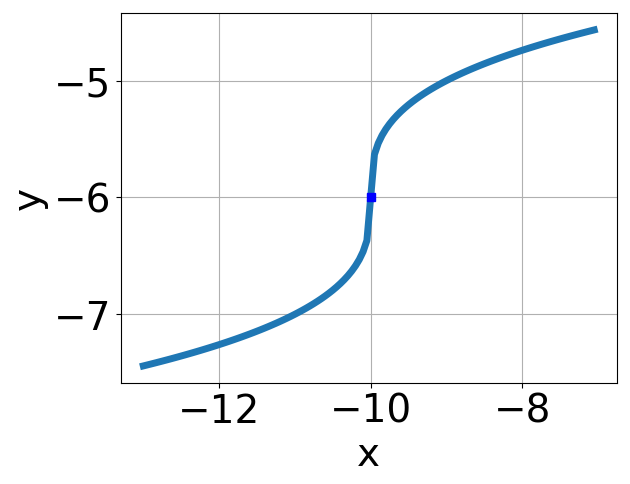
\includegraphics[width = 0.3\textwidth]{../Figures/radicalEquationToGraphAC.png}\item 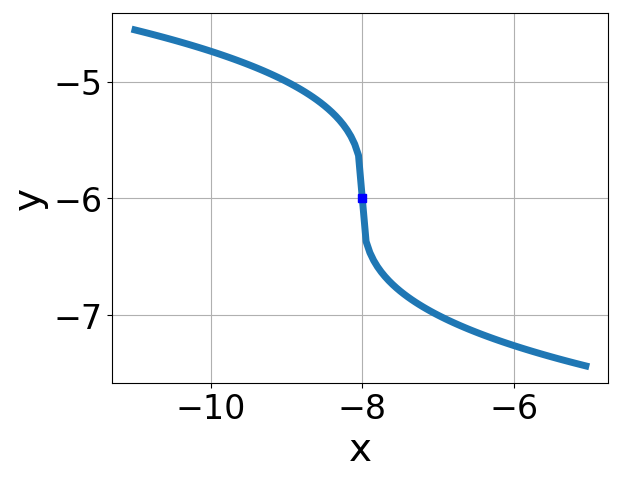
\includegraphics[width = 0.3\textwidth]{../Figures/radicalEquationToGraphBC.png}\item 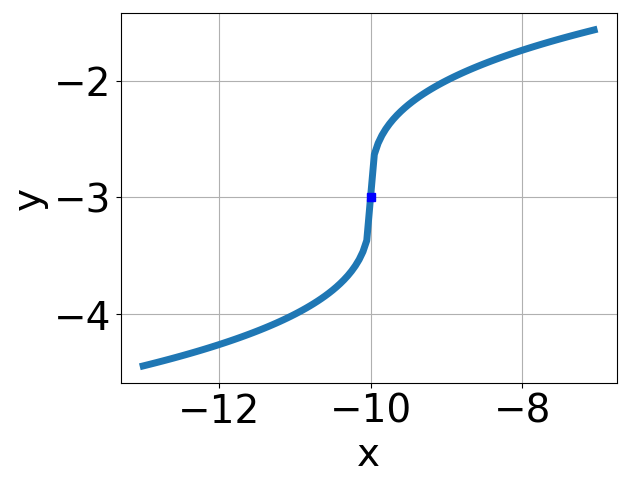
\includegraphics[width = 0.3\textwidth]{../Figures/radicalEquationToGraphCC.png}\item 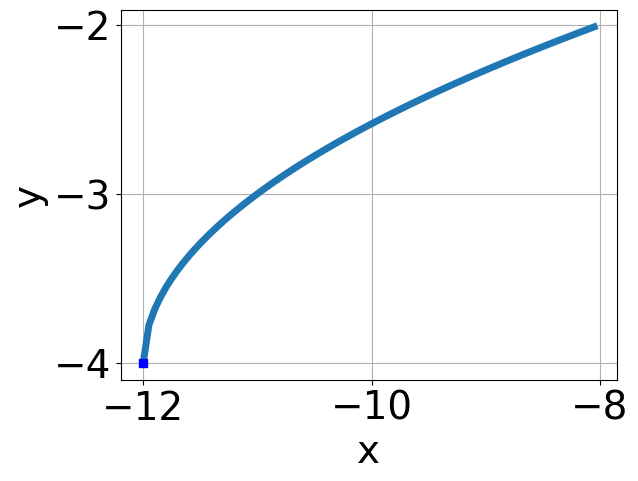
\includegraphics[width = 0.3\textwidth]{../Figures/radicalEquationToGraphDC.png}\end{multicols}\item None of the above.
\end{enumerate} }
\litem{
Choose the equation of the function graphed below.
\begin{center}
    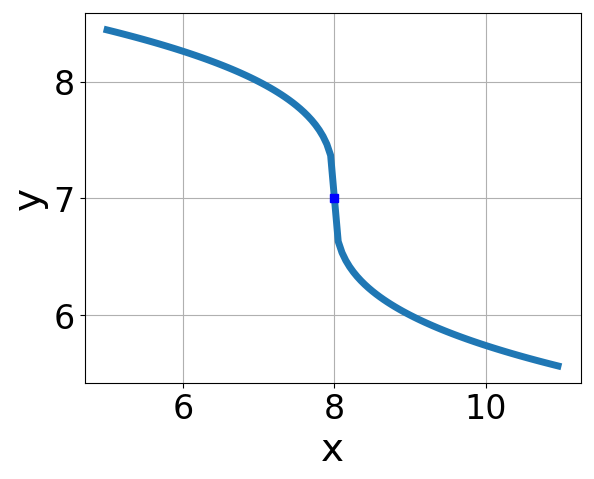
\includegraphics[width=0.5\textwidth]{../Figures/radicalGraphToEquationC.png}
\end{center}
\begin{enumerate}[label=\Alph*.]
\item \( f(x) = \sqrt[3]{x + 10} + 6 \)
\item \( f(x) = - \sqrt[3]{x - 10} + 6 \)
\item \( f(x) = - \sqrt[3]{x + 10} + 6 \)
\item \( f(x) = \sqrt[3]{x - 10} + 6 \)
\item \( \text{None of the above} \)

\end{enumerate} }
\litem{
Choose the equation of the function graphed below.
\begin{center}
    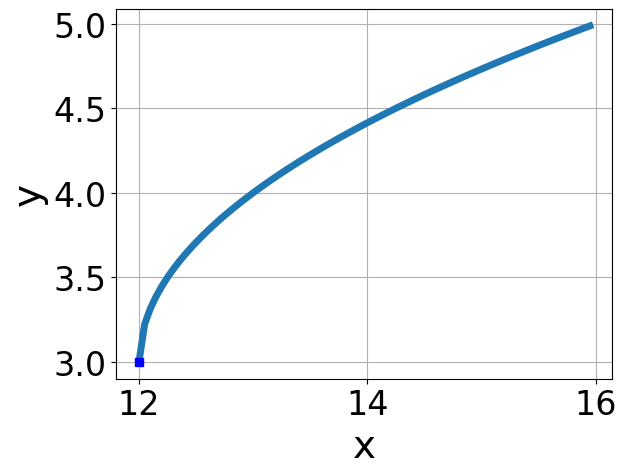
\includegraphics[width=0.5\textwidth]{../Figures/radicalGraphToEquationCopyC.png}
\end{center}
\begin{enumerate}[label=\Alph*.]
\item \( f(x) = \sqrt[3]{x - 6} + 5 \)
\item \( f(x) = \sqrt[3]{x + 6} + 5 \)
\item \( f(x) = - \sqrt[3]{x - 6} + 5 \)
\item \( f(x) = - \sqrt[3]{x + 6} + 5 \)
\item \( \text{None of the above} \)

\end{enumerate} }
\litem{
Solve the radical equation below. Then, choose the interval(s) that the solution(s) belongs to.\[ \sqrt{-2 x + 8} - \sqrt{-6 x + 7} = 0 \]\begin{enumerate}[label=\Alph*.]
\item \( x \in [-6.3,-3.3] \)
\item \( x \in [-2.3,0.3] \)
\item \( \text{All solutions lead to invalid or complex values in the equation.} \)
\item \( x_1 \in [-2.3, 0.3] \text{ and } x_2 \in [4,5] \)
\item \( x_1 \in [0, 2.3] \text{ and } x_2 \in [4,5] \)

\end{enumerate} }
\litem{
What is the domain of the function below?\[ f(x) = \sqrt[4]{-5 x + 4} \]\begin{enumerate}[label=\Alph*.]
\item \( (-\infty, a], \text{ where } a \in [0.75, 0.96] \)
\item \( (-\infty, \infty) \)
\item \( [a, \infty), \text{where } a \in [0.29, 1.23] \)
\item \( (-\infty, a], \text{where } a \in [0.98, 1.43] \)
\item \( [a, \infty), \text{where } a \in [1, 1.39] \)

\end{enumerate} }
\litem{
What is the domain of the function below?\[ f(x) = \sqrt[3]{7 x - 3} \]\begin{enumerate}[label=\Alph*.]
\item \( \text{The domain is } [a, \infty), \text{   where } a \in [-0.57, 1.43] \)
\item \( (-\infty, \infty) \)
\item \( \text{The domain is } (-\infty, a], \text{   where } a \in [1.44, 3.87] \)
\item \( \text{The domain is } (-\infty, a], \text{   where } a \in [0.31, 1.31] \)
\item \( \text{The domain is } [a, \infty), \text{   where } a \in [2.33, 6.33] \)

\end{enumerate} }
\litem{
Solve the radical equation below. Then, choose the interval(s) that the solution(s) belongs to.\[ \sqrt{-6 x^2 - 27} - \sqrt{33 x} = 0 \]\begin{enumerate}[label=\Alph*.]
\item \( x_1 \in [-7.5, -1.5] \text{ and } x_2 \in [-2.8,0.3] \)
\item \( x_1 \in [4.5, 6.5] \text{ and } x_2 \in [0.3,2.4] \)
\item \( \text{All solutions lead to invalid or complex values in the equation.} \)
\item \( x \in [-7.5,-1.5] \)
\item \( x \in [-1,1] \)

\end{enumerate} }
\litem{
Choose the graph of the equation below.\[ f(x) = \sqrt[3]{x - 12} - 3 \]\begin{enumerate}[label=\Alph*.]
\begin{multicols}{2}\item 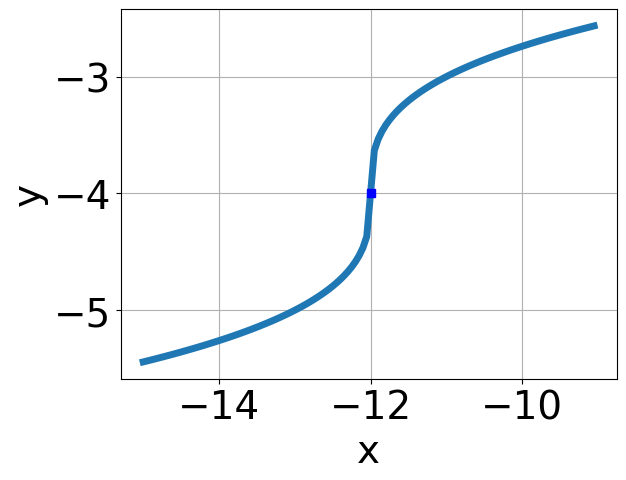
\includegraphics[width = 0.3\textwidth]{../Figures/radicalEquationToGraphCopyAC.png}\item 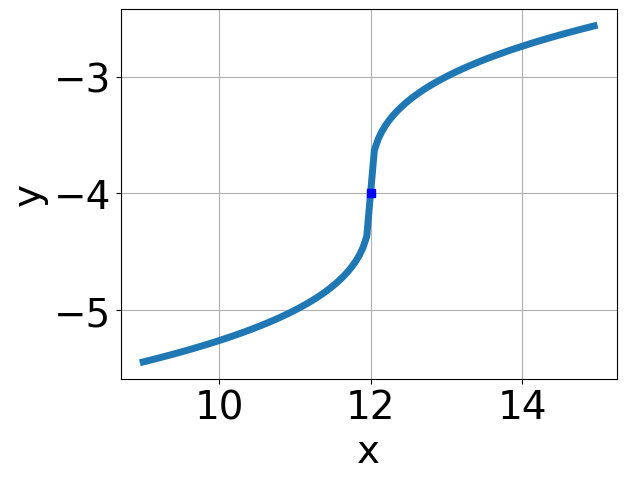
\includegraphics[width = 0.3\textwidth]{../Figures/radicalEquationToGraphCopyBC.png}\item 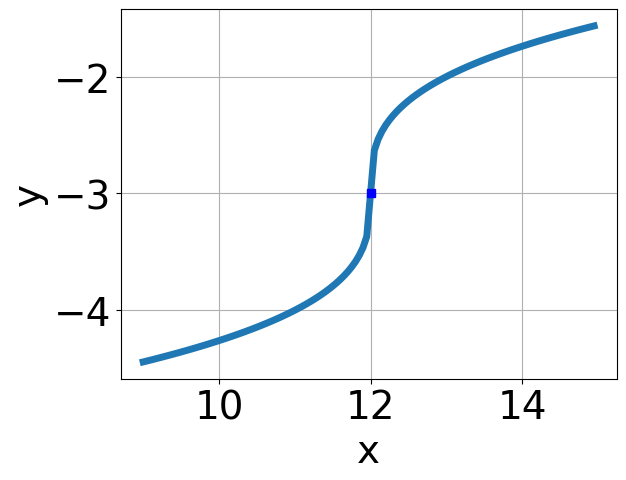
\includegraphics[width = 0.3\textwidth]{../Figures/radicalEquationToGraphCopyCC.png}\item 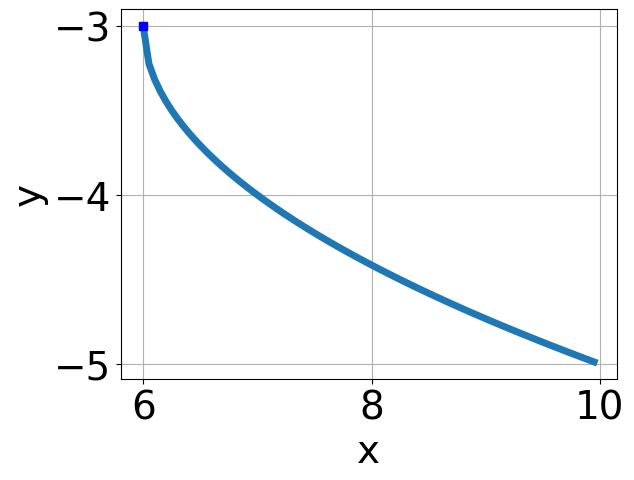
\includegraphics[width = 0.3\textwidth]{../Figures/radicalEquationToGraphCopyDC.png}\end{multicols}\item None of the above.
\end{enumerate} }
\end{enumerate}

\end{document}